%  LaTeX support: latex@mdpi.com 
%  For support, please attach all files needed for compiling as well as the log file, and specify your operating system, LaTeX version, and LaTeX editor.

%=================================================================
\documentclass[software,article,submit,pdftex,moreauthors]{Definitions/mdpi}
\usepackage[dvipsnames]{xcolor}
\usepackage{listings}

\lstdefinelanguage{Kotlin}{
  comment=[l]{//},
  commentstyle={\color{gray}\ttfamily},
  emph={filter, first, firstOrNull, forEach, lazy, map, mapNotNull, println},
  emphstyle={\color{OrangeRed}},
  identifierstyle=\color{black},
  keywords={!in, !is, abstract, actual, annotation, as, as?, break, by, catch, class, companion, const, constructor, continue, crossinline, data, delegate, do, dynamic, else, enum, expect, external, false, field, file, final, finally, for, fun, get, if, import, in, infix, init, inline, inner, interface, internal, is, lateinit, noinline, null, object, open, operator, out, override, package, param, private, property, protected, public, receiver, reified, return, return@, sealed, set, setparam, super, suspend, tailrec, this, throw, true, try, typealias, typeof, val, var, vararg, when, where, while},
  keywordstyle={\color{NavyBlue}\bfseries},
  escapeinside={//(`}{`)},
  morecomment=[s]{/*}{*/},
  morestring=[b]",
  morestring=[s]{"""*}{*"""},
  ndkeywords={@Composable, @Preview, @Deprecated, @JvmField, @JvmName, @JvmOverloads, @JvmStatic, @JvmSynthetic, Array, Byte, Double, Float, Int, Integer, Iterable, Long, Runnable, Short, String, Any, Unit, Nothing},
  ndkeywordstyle={\color{BurntOrange}\bfseries},
  sensitive=true,
  stringstyle={\color{ForestGreen}\ttfamily},
}

%\documentclass[preprints,article,submit,pdftex,moreauthors]{Definitions/mdpi} 
% For posting an early version of this manuscript as a preprint, you may use "preprints" as the journal. Changing "submit" to "accept" before posting will remove line numbers.

% Below journals will use APA reference format:
% admsci, behavsci, businesses, econometrics, economies, education, ejihpe, famsci, games, humans, ijcs, ijfs, journalmedia, jrfm, languages, psycholint, publications, tourismhosp, youth

% Below journals will use Chicago reference format:
% arts, genealogy, histories, humanities, jintelligence, laws, literature, religions, risks, socsci

%--------------------
% Class Options:
%--------------------
%----------
% journal
%----------
% Choose between the following MDPI journals:
% accountaudit, acoustics, actuators, addictions, adhesives, admsci, adolescents, aerobiology, aerospace, agriculture, agriengineering, agrochemicals, agronomy, ai, air, algorithms, allergies, alloys, amh, analytica, analytics, anatomia, anesthres, animals, antibiotics, antibodies, antioxidants, applbiosci, appliedchem, appliedmath, appliedphys, applmech, applmicrobiol, applnano, applsci, aquacj, architecture, arm, arthropoda, arts, asc, asi, astronomy, atmosphere, atoms, audiolres, automation, axioms, bacteria, batteries, bdcc, behavsci, beverages, biochem, bioengineering, biologics, biology, biomass, biomechanics, biomed, biomedicines, biomedinformatics, biomimetics, biomolecules, biophysica, biosensors, biosphere, biotech, birds, blockchains, bloods, blsf, brainsci, breath, buildings, businesses, cancers, carbon, cardiogenetics, catalysts, cells, ceramics, challenges, chemengineering, chemistry, chemosensors, chemproc, children, chips, cimb, civileng, cleantechnol, climate, clinbioenerg, clinpract, clockssleep, cmd, cmtr, coasts, coatings, colloids, colorants, commodities, complications, compounds, computation, computers, condensedmatter, conservation, constrmater, cosmetics, covid, crops, cryo, cryptography, crystals, csmf, ctn, curroncol, cyber, dairy, data, ddc, dentistry, dermato, dermatopathology, designs, devices, diabetology, diagnostics, dietetics, digital, disabilities, diseases, diversity, dna, drones, dynamics, earth, ebj, ecm, ecologies, econometrics, economies, education, eesp, ejihpe, electricity, electrochem, electronicmat, electronics, encyclopedia, endocrines, energies, eng, engproc, ent, entomology, entropy, environments, epidemiologia, epigenomes, esa, est, famsci, fermentation, fibers, fintech, fire, fishes, fluids, foods, forecasting, forensicsci, forests, fossstud, foundations, fractalfract, fuels, future, futureinternet, futureparasites, futurepharmacol, futurephys, futuretransp, galaxies, games, gases, gastroent, gastrointestdisord, gastronomy, gels, genealogy, genes, geographies, geohazards, geomatics, geometry, geosciences, geotechnics, geriatrics, glacies, grasses, greenhealth, gucdd, hardware, hazardousmatters, healthcare, hearts, hemato, hematolrep, heritage, higheredu, highthroughput, histories, horticulturae, hospitals, humanities, humans, hydrobiology, hydrogen, hydrology, hygiene, idr, iic, ijerph, ijfs, ijgi, ijmd, ijms, ijns, ijpb, ijt, ijtm, ijtpp, ime, immuno, informatics, information, infrastructures, inorganics, insects, instruments, inventions, iot, j, jal, jcdd, jcm, jcp, jcs, jcto, jdad, jdb, jeta, jfb, jfmk, jimaging, jintelligence, jlpea, jmahp, jmmp, jmms, jmp, jmse, jne, jnt, jof, joitmc, joma, jop, jor, journalmedia, jox, jpbi, jpm, jrfm, jsan, jtaer, jvd, jzbg, kidney, kidneydial, kinasesphosphatases, knowledge, labmed, laboratories, land, languages, laws, life, lights, limnolrev, lipidology, liquids, literature, livers, logics, logistics, lubricants, lymphatics, machines, macromol, magnetism, magnetochemistry, make, marinedrugs, materials, materproc, mathematics, mca, measurements, medicina, medicines, medsci, membranes, merits, metabolites, metals, meteorology, methane, metrics, metrology, micro, microarrays, microbiolres, microelectronics, micromachines, microorganisms, microplastics, microwave, minerals, mining, mmphys, modelling, molbank, molecules, mps, msf, mti, multimedia, muscles, nanoenergyadv, nanomanufacturing, nanomaterials, ncrna, ndt, network, neuroglia, neurolint, neurosci, nitrogen, notspecified, nursrep, nutraceuticals, nutrients, obesities, oceans, ohbm, onco, oncopathology, optics, oral, organics, organoids, osteology, oxygen, parasites, parasitologia, particles, pathogens, pathophysiology, pediatrrep, pets, pharmaceuticals, pharmaceutics, pharmacoepidemiology, pharmacy, philosophies, photochem, photonics, phycology, physchem, physics, physiologia, plants, plasma, platforms, pollutants, polymers, polysaccharides, populations, poultry, powders, preprints, proceedings, processes, prosthesis, proteomes, psf, psych, psychiatryint, psychoactives, psycholint, publications, purification, quantumrep, quaternary, qubs, radiation, reactions, realestate, receptors, recycling, regeneration, religions, remotesensing, reports, reprodmed, resources, rheumato, risks, robotics, rsee, ruminants, safety, sci, scipharm, sclerosis, seeds, sensors, separations, sexes, signals, sinusitis, siuj, skins, smartcities, sna, societies, socsci, software, soilsystems, solar, solids, spectroscj, sports, standards, stats, std, stresses, surfaces, surgeries, suschem, sustainability, symmetry, synbio, systems, tae, targets, taxonomy, technologies, telecom, test, textiles, thalassrep, therapeutics, thermo, timespace, tomography, tourismhosp, toxics, toxins, transplantology, transportation, traumacare, traumas, tropicalmed, universe, urbansci, uro, vaccines, vehicles, venereology, vetsci, vibration, virtualworlds, viruses, vision, waste, water, wem, wevj, wild, wind, women, world, youth, zoonoticdis

%---------
% article
%---------
% The default type of manuscript is "article", but can be replaced by: 
% abstract, addendum, article, benchmark, book, bookreview, briefcommunication, briefreport, casereport, changes, clinicopathologicalchallenge, comment, commentary, communication, conceptpaper, conferenceproceedings, correction, conferencereport, creative, datadescriptor, discussion, entry, expressionofconcern, extendedabstract, editorial, essay, erratum, fieldguide, hypothesis, interestingimages, letter, meetingreport, monograph, newbookreceived, obituary, opinion, proceedingpaper, projectreport, reply, retraction, review, perspective, protocol, shortnote, studyprotocol, supfile, systematicreview, technicalnote, viewpoint, guidelines, registeredreport, tutorial,  giantsinurology, urologyaroundtheworld
% supfile = supplementary materials

%----------
% submit
%----------
% The class option "submit" will be changed to "accept" by the Editorial Office when the paper is accepted. This will only make changes to the frontpage (e.g., the logo of the journal will get visible), the headings, and the copyright information. Also, line numbering will be removed. Journal info and pagination for accepted papers will also be assigned by the Editorial Office.

%------------------
% moreauthors
%------------------
% If there is only one author the class option oneauthor should be used. Otherwise use the class option moreauthors.

%---------
% pdftex
%---------
% The option pdftex is for use with pdfLaTeX. Remove "pdftex" for (1) compiling with LaTeX & dvi2pdf (if eps figures are used) or for (2) compiling with XeLaTeX.

%=================================================================
% MDPI internal commands - do not modify
\firstpage{1} 
\makeatletter 
\setcounter{page}{\@firstpage} 
\makeatother
\pubvolume{1}
\issuenum{1}
\articlenumber{0}
\pubyear{2025}
\copyrightyear{2025}
%\externaleditor{Firstname Lastname} % More than 1 editor, please add `` and '' before the last editor name
\datereceived{ } 
\daterevised{ } % Comment out if no revised date
\dateaccepted{ } 
\datepublished{ } 
%\datecorrected{} % For corrected papers: "Corrected: XXX" date in the original paper.
%\dateretracted{} % For retracted papers: "Retracted: XXX" date in the original paper.
\hreflink{https://doi.org/} % If needed use \linebreak
%\doinum{}
%\pdfoutput=1 % Uncommented for upload to arXiv.org
%\CorrStatement{yes}  % For updates
%\longauthorlist{yes} % For many authors that exceed the left citation part

%=================================================================
% Add packages and commands here. The following packages are loaded in our class file: fontenc, inputenc, calc, indentfirst, fancyhdr, graphicx, epstopdf, lastpage, ifthen, float, amsmath, amssymb, lineno, setspace, enumitem, mathpazo, booktabs, titlesec, etoolbox, tabto, xcolor, colortbl, soul, multirow, microtype, tikz, totcount, changepage, attrib, upgreek, array, tabularx, pbox, ragged2e, tocloft, marginnote, marginfix, enotez, amsthm, natbib, hyperref, cleveref, scrextend, url, geometry, newfloat, caption, draftwatermark, seqsplit
% cleveref: load \crefname definitions after \begin{document}

%=================================================================
% Please use the following mathematics environments: Theorem, Lemma, Corollary, Proposition, Characterization, Property, Problem, Example, ExamplesandDefinitions, Hypothesis, Remark, Definition, Notation, Assumption
%% For proofs, please use the proof environment (the amsthm package is loaded by the MDPI class).

%=================================================================
% Full title of the paper (Capitalized)
\Title{Non-blocking Progressive Server-side Rendering (PSSR) Benchmark}

% MDPI internal command: Title for citation in the left column
\TitleCitation{Non-blocking Progressive Server-side Rendering (PSSR) Benchmark}

% Author Orchid ID: enter ID or remove command
\newcommand{\orcidauthorA}{0000-0000-0000-000X} % Add \orcidA{} behind the author's name
%\newcommand{\orcidauthorB}{0000-0000-0000-000X} % Add \orcidB{} behind the author's name

% Authors, for the paper (add full first names)
\Author{Bernardo Pereira $^{1,*}$\orcidA{}, Miguel Carvalho $^{2}$ \orcidA{}}

%\longauthorlist{yes}

% MDPI internal command: Authors, for metadata in PDF
\AuthorNames{Bernardo Pereira, Miguel Carvalho}

% MDPI internal command: Authors, for citation in the left column, only choose below one of them according to the journal style
% If this is a Chicago style journal 
% (arts, genealogy, histories, humanities, jintelligence, laws, literature, religions, risks, socsci): 
% Lastname, Firstname, Firstname Lastname, and Firstname Lastname.

% If this is a APA style journal 
% (admsci, behavsci, businesses, econometrics, economies, education, ejihpe, games, humans, ijfs, journalmedia, jrfm, languages, psycholint, publications, tourismhosp, youth): 
% Lastname, F., Lastname, F., \& Lastname, F.

% If this is a ACS style journal (Except for the above Chicago and APA journals, all others are in the ACS format): 
% Lastname, F.; Lastname, F.; Lastname, F.
% \isAPAStyle{%
%        \AuthorCitation{Lastname, F., Lastname, F., \& Lastname, F.}
%          }{%
%         \isChicagoStyle{%
%         \AuthorCitation{Lastname, Firstname, Firstname Lastname, and Firstname Lastname.}
%         }{
%         \AuthorCitation{Lastname, F.; Lastname, F.; Lastname, F.}
%         }
% }

% Affiliations / Addresses (Add [1] after \address if there is only one affiliation.)
\address[1]{%
$^{1}$ \quad Instituto Superior de Engenharia de Lisboa, Instituto Politécnico de Lisboa, 1950-062 Lisbon, Portugal\\}


% Contact information of the corresponding author
\corres{Author to whom correspondence should be addressed.}

% Current address and/or shared authorship
% \firstnote{Current address: Affiliation.}  % Current address should not be the same as any items in the Affiliation section.

% The commands \thirdnote{} till \eighthnote{} are available for further notes

%\simplesumm{} % Simple summary

%\conference{} % An extended version of a conference paper

% Abstract (Do not insert blank lines, i.e. \\) 
\abstract{A single paragraph of about 200 words maximum. For research articles, abstracts should give a pertinent overview of the work. We strongly encourage authors to use the following style of structured abstracts, but without headings: (1) Background: place the question addressed in a broad context and highlight the purpose of the study; (2) Methods: describe briefly the main methods or treatments applied; (3) Results: summarize the article's main findings; (4) Conclusions: indicate the main conclusions or interpretations. The abstract should be an objective representation of the article, it must not contain results which are not presented and substantiated in the main text and should not exaggerate the main conclusions.}

% Keywords
\keyword{keyword 1; keyword 2; keyword 3 (List three to ten pertinent keywords specific to the article; yet reasonably common within the subject discipline.)} 

% The fields PACS, MSC, and JEL may be left empty or commented out if not applicable
%\PACS{J0101}
%\MSC{}
%\JEL{}

%%%%%%%%%%%%%%%%%%%%%%%%%%%%%%%%%%%%%%%%%%
% Only for the journal Diversity
%\LSID{\url{http://}}

%%%%%%%%%%%%%%%%%%%%%%%%%%%%%%%%%%%%%%%%%%
% Only for the journal Applied Sciences
%\featuredapplication{Authors are encouraged to provide a concise description of the specific application or a potential application of the work. This section is not mandatory.}
%%%%%%%%%%%%%%%%%%%%%%%%%%%%%%%%%%%%%%%%%%

%%%%%%%%%%%%%%%%%%%%%%%%%%%%%%%%%%%%%%%%%%
% Only for the journal Data
%\dataset{DOI number or link to the deposited data set if the data set is published separately. If the data set shall be published as a supplement to this paper, this field will be filled by the journal editors. In this case, please submit the data set as a supplement.}
%\datasetlicense{License under which the data set is made available (CC0, CC-BY, CC-BY-SA, CC-BY-NC, etc.)}

%%%%%%%%%%%%%%%%%%%%%%%%%%%%%%%%%%%%%%%%%%
% Only for the journal Toxins
%\keycontribution{The breakthroughs or highlights of the manuscript. Authors can write one or two sentences to describe the most important part of the paper.}

%%%%%%%%%%%%%%%%%%%%%%%%%%%%%%%%%%%%%%%%%%
% Only for the journal Encyclopedia
%\encyclopediadef{For entry manuscripts only: please provide a brief overview of the entry title instead of an abstract.}

%%%%%%%%%%%%%%%%%%%%%%%%%%%%%%%%%%%%%%%%%%
% Only for the journal Advances in Respiratory Medicine, Smart Cities and Sensors
%\addhighlights{yes}
%\renewcommand{\addhighlights}{%
%
%\noindent This is an obligatory section in “Advances in Respiratory Medicine'' and ``Smart Cities”, whose goal is to increase the discoverability and readability of the article via search engines and other scholars. Highlights should not be a copy of the abstract, but a simple text allowing the reader to quickly and simplified find out what the article is about and what can be cited from it. Each of these parts should be devoted up to 2~bullet points.\vspace{3pt}\\
%\textbf{What are the main findings?}
% \begin{itemize}[labelsep=2.5mm,topsep=-3pt]
% \item First bullet.
% \item Second bullet.
% \end{itemize}\vspace{3pt}
%\textbf{What is the implication of the main finding?}
% \begin{itemize}[labelsep=2.5mm,topsep=-3pt]
% \item First bullet.
% \item Second bullet.
% \end{itemize}
%}

%%%%%%%%%%%%%%%%%%%%%%%%%%%%%%%%%%%%%%%%%%
\begin{document}

%%%%%%%%%%%%%%%%%%%%%%%%%%%%%%%%%%%%%%%%%%

\documentclass[../ppG48.tex]{subfiles}

\begin{document}

Non-blocking Progressive Server-Side Rendering (PSSR) is a technique that combines some of the advantages of both server-side and client-side rendering to improve web application performance and user experience. By leveraging non-blocking I/O operations, PSSR allows for efficient handling of multiple concurrent requests while progressively streaming HTML content to the client.

This project consists of a benchmark that evaluates the performance of different PSSR strategies on the Java Virtual Machine (JVM). The benchmark focuses on evaluating the performance of non-blocking PSSR implementations using approaches such as Kotlin coroutines, reactive-style programming, and Java virtual threads. Its main objective is to evaluate virtual threads as an alternative that ensures a non-blocking approach to PSSR while offering a more straightforward programming model than traditional asynchronous programming techniques.

This project aims to extend the previous work done in \textit{spring-webflux-comparing-template-engines} \cite{spring-webflux-comparing-template-engines}, which compares the performance of various template engines in a Spring WebFlux application using different approaches to PSSR. It adds support for Java virtual threads and evaluates non-blocking PSSR implementations in other frameworks compared to Spring WebFlux.

Currently, this project features a working benchmark in Spring WebFlux, Spring MVC, and Quarkus, comparing the performance of eight different template engines: Rocker, JStachio, Pebble, Freemarker, Trimou, Thymeleaf, HtmlFlow, and KotlinX. It includes Java Microbenchmark Harness (JMH) benchmarks for template engine performance testing, as well as Apache Bench and Apache JMeter scripts for evaluating throughput and scalability. In the future, the project could be extended to include other frameworks such as Vert.x, if time allows. However, the next objective is the completion of the written report and article submission. The written report will include a more detailed analysis of the benchmark results, along with a contextualization of the state of the art in non-blocking PSSR and asynchronous programming.

This report will focus on detailing relevant aspects of the benchmark implementation and methodology, and will also provide a brief overview of the results obtained from the JMeter and Apache Bench tests, which evaluate the throughput and scalability of the different implementations.

\end{document}


% The introduction should briefly place the study in a broad context and
% highlight why it is important. It should define the purpose of the work and its
% significance. The current state of the research field should be reviewed
% carefully and key publications cited. Please highlight controversial and
% diverging hypotheses when necessary. Finally, briefly mention the main aim of
% the work and highlight the principal conclusions. As far as possible, please
% keep the introduction comprehensible to scientists outside your particular
% field of research. Citing a journal paper \citep{ref-journal}. Now citing a
% book reference \citep{ref-book1,ref-book2} or other reference types
% \citep{ref-unpublish,ref-url}. Please use the command
% \citep{ref-proceeding,ref-thesis} for the following MDPI journals, which use
% author--date citation: Administrative Sciences, Arts, Behavioral Sciences,
% Businesses, Econometrics, Economies, Education Sciences, European Journal of
% Investigation in Health, Psychology and Education, Games, Genealogy, Histories,
% Humanities, Humans, IJFS, Journal of Intelligence, Journalism and Media, JRFM,
% Languages, Laws, Literature, Psychology International, Publications, Religions,
% Risks, Social Sciences, Tourism and Hospitality, Youth.}

%%%%%%%%%%%%%%%%%%%%%%%%%%%%%%%%%%%%%%%%%%
\section{Background and Related Work}

In this section, we first examine the different design choices adopted by web 
servers in their internal architectures, and how these choices impact the 
behavior of the web template engines.
Then, in Subsection~2.2, we present the main properties that characterize each 
web template technology approach, along with the advantages and drawbacks that 
result from these characteristics.

%%%%%%%%%%%%%%%%%%%%%%%%%%%%%%%%%%%%%%%%%%%%%%%%%%%%%%%%%%%%%%%%%%%%
%-------------------------------------------------------------------
%%%%%%%%%%%%%%%%%%%%%%%%%%%%%%%%%%%%%%%%%%%%%%%%%%%%%%%%%%%%%%%%%%%%

\subsection{Web Framework Architectures and Approaches to PSSR}

In traditional thread-per-request architectures, each incoming request is
handled by a dedicated thread. The web server maintains a thread pool from
which a thread is assigned to handle each request. As the load increases, the
number of active threads can grow rapidly, potentially exhausting the pool.
This can lead to performance and scalability issues, as the system may become
bogged down by context switching and thread management
overhead~\cite{kant2000scalable}.
In the Java ecosystem, Spring Boot is one of the most widely used frameworks that
follow this model, according to several reports such as the Stack Overflow 2024
Developer
Survey~\footnote{~\url{https://survey.stackoverflow.co/2024/technology\#1-web-frameworks-and-technologies}}.

On the other hand, in modern \textit{low-thread} architectures, the server uses
a small number of threads to handle a large number of requests.
\textit{Low-thread} servers, also known as
\textit{event-driven}~\cite{event-driven-servers}, offer a significant
advantage in efficiently managing a high number of concurrent I/O operations
with minimal resource usage.

The \textit{non-blocking} I/O model employed in low-thread servers is
well-suited for handling large volumes of data asynchronously~\cite{Meijer12}.
This combination of low-thread servers and asynchronous data models has
facilitated the development of highly scalable, responsive, and resilient web
applications capable of managing substantial data loads~\cite{Jin15}.
The prominence of this concept increased with the advent of Node.js in
2009, and subsequently, various technologies adopted this approach
in the Java ecosystem, including Netty, Akka HTTP, Vert.X, and Spring WebFlux.
% Among these, Spring WebFlux stands out as the most widely used web framework in
% Java, according to surveys like JetBrains' State of Java report (2021) and
% community metrics from platforms like Github and StackOverflow.
The \textit{non-blocking} I/O model in low-thread servers functions optimally
only when HTTP handlers avoid blocking.
Therefore, HTML templates need to be proficient in dealing with the asynchronous
APIs provided by data models.
While most legacy web templates struggle with asynchronous models, DSLs for HTML
face no such limitations, leveraging all constructions available in the host
programming language.
However, the unexpected intertwining of asynchronous handlers' completion and
HTML builders' execution may potentially lead to malformed HTML with an
unexpected layout, as demonstrated in the subsequent subsection~\ref{sec:async-support}.

An alternative approach involves utilizing user-level threads, while maintaining
a blocking I/O and a synchronous programming paradigm.
However, this approach still requires a user-level I/O subsystem capable of
mitigating system-level blocking, which is crucial for the performance of
I/O-intensive applications. This technique offers a lightweight solution for
efficiently managing a larger number of concurrent sessions by minimizing
per-thread overhead.
In 2020, Karsten~\cite{karsten2020} demonstrated how this strategy supports a
synchronous programming style, effectively abstracting away the complexities
associated with managing continuations in asynchronous programming.

Among mainstream technologies, the Kotlin programming language introduces a new 
abstraction for managing coroutines and provides structured concurrency, which 
ensures that coroutines are \textit{scoped}, \textit{cancellable}, and 
\textit{coordinated} within a well-defined 
lifecycle~\cite{elizarov2021coroutines}.
Although this model embraces the \texttt{async}/\texttt{await}
feature~\cite{async_await}, enabling non-blocking routines to mimic the
structure of synchronous ones, it still lacks a user-level I/O subsystem and
relies on an explicit I/O dispatcher tied to a dedicated thread pool that frees
worker threads for handling processing tasks.
Moreover, web templates using their own templating dialects, such as JSP, 
Thymeleaf, or Handlebars, are unable to take advantage of such constructs, as 
they typically support only a limited subset of the host library's API—most 
commonly just the \texttt{Iterable} interface.

Only Java virtual threads, introduced in
JEP~444~\footnote{\url{https://openjdk.org/jeps/444}}, adopt a similar approach
to Karsten's proposal, using user-mode threads to preserve a synchronous
programming model while still allowing blocking I/O operations without tying up
platform threads. When a virtual thread performs a blocking I/O operation, the
JVM intercepts the call and transparently parks the virtual thread, freeing the
underlying platform thread to perform other tasks. Once the I/O operation
completes, the virtual thread is rescheduled on a platform thread and resumes
execution. This mechanism is enabled by the JVM's integration with non-blocking
system calls at the OS level, allowing developers to write traditional
synchronous code while benefiting from the scalability of non-blocking I/O.


\subsubsection{Spring MVC}

\subsubsection{Spring WebFlux}

\subsubsection{Quarkus}

%%%%%%%%%%%%%%%%%%%%%%%%%%%%%%%%%%%%%%%%%%%%%%%%%%%%%%%%%%%%%%%%%%%%
%-------------------------------------------------------------------
%%%%%%%%%%%%%%%%%%%%%%%%%%%%%%%%%%%%%%%%%%%%%%%%%%%%%%%%%%%%%%%%%%%%

\subsection{Web Templates}

\textit{Web templates} have been the most widely adopted approach for
constructing dynamic HTML pages.
Web templates or \textit{web views}~\cite{Fowler02,Alur01} (e.g. JSP, Handlebars,
or Thymeleaf), are based on HTML documents augmented with template-specific
markers (e.g., \texttt{<\%>}, \texttt{\{\{\}\}}, or \texttt{\$\{\}}), which
represent \textit{dynamic} information to be replaced at runtime with the
results of corresponding computations, producing the final HTML page.
The process of parsing and replacing these markers---i.e.,
\textit{resolution}---is the primary responsibility of the \textit{template
engine}~\cite{Parr04}.
One key characteristic of \textit{web templates} is their ability to receive a 
\textit{context object}---equivalent to the \textit{model} in the model-view 
design pattern~\cite{mvc88,Parr04}---which provides the data used to fill 
template placeholders at runtime.
Web templates can be distinguished by several properties, namely:
\begin{enumerate}
    \item \textit{Domain-specific language} idiom
    \item Supported data model APIs
    \item Asynchronous support
    \item Type safety and HTML safety
    \item Progressive rendering
\end{enumerate}

Although some of the aforementioned characteristics apply to both \textit{server-side}
and \textit{client-side} approaches, we focus solely on web template technologies for
\textit{server-side rendering}, as our work is centered on that approach.
Before getting deep on each of the aforementioned characteristics,
Table~\ref{table:cmplibs} presents a breakdown of mainstream template engines,
classified according to the identified properties.

\begin{table}[h]
  \small
	\tabcolsep=0.1cm
	\def\arraystretch{1.2}
	\begin{tabular}{|c|c|c|c|c|c|c|}
		\hline                                                                  
		\textbf{Library}
		&\textbf{DSL idiom}
		&\textbf{Data Model APIs}
    &\shortstack{\textbf{Asynchronous}\\\textbf{Support}}
    &\shortstack{\textbf{Type}\\\textbf{Safety}}
    &\shortstack{\textbf{HTML}\\\textbf{Safety}}
		&\shortstack{\textbf{Progressive}\\\textbf{Rendering}}
		\\
		\hline
		\textbf{Freemarker}
		&External DSL
		&\texttt{Iterable}
		&\large{$\textcolor{red}{\times}$}
    &\large{$\textcolor{red}{\times}$}
    &\large{$\textcolor{red}{\times}$}
		&\large{$\textcolor{PineGreen}{\checkmark}$}
		\\
    \hline
		\textbf{JSP}
		&External DSL
		&\texttt{Iterable}
		&\large{$\textcolor{red}{\times}$}
    &\large{$\textcolor{red}{\times}$}
    &\large{$\textcolor{red}{\times}$}
		&\large{$\textcolor{red}{\times}$}
    \\
    \hline
		\textbf{JStachio}
		&External DSL
		&\texttt{Iterable}
		&\large{$\textcolor{red}{\times}$}
    &\large{$\textcolor{red}{\times}$}
    &\large{$\textcolor{red}{\times}$}
		&\large{$\textcolor{PineGreen}{\checkmark}$}
		\\\hline
		\textbf{Pebble}
		&External DSL
		&\texttt{Iterable}
		&\large{$\textcolor{red}{\times}$}
    &\large{$\textcolor{red}{\times}$}
    &\large{$\textcolor{red}{\times}$}
		&\large{$\textcolor{PineGreen}{\checkmark}$}
		\\
    \hline
		\textbf{Rocker}
		&External DSL
		&\texttt{Iterable}
		&\large{$\textcolor{red}{\times}$}
    &\large{$\textcolor{red}{\times}$}
    &\large{$\textcolor{red}{\times}$}
		&\large{$\textcolor{PineGreen}{\checkmark}$}
		\\
    \hline
		\textbf{Thymeleaf}
		&External DSL
		&\shortstack{\texttt{Iterable}\\\texttt{Publisher}}
		&\texttt{Publisher}$^{(1)}$
    &\large{$\textcolor{red}{\times}$}
    &\large{$\textcolor{red}{\times}$}
		&\large{$\textcolor{PineGreen}{\checkmark}$}
		\\
    \hline
		\textbf{Trimou}
		&External DSL
		&\texttt{Iterable}
		&\large{$\textcolor{red}{\times}$}
    &\large{$\textcolor{red}{\times}$}
    &\large{$\textcolor{red}{\times}$}
		&\large{$\textcolor{PineGreen}{\checkmark}$}
		\\
    \hline
		\textbf{Velocity}
		&External DSL
		&\texttt{Iterable}
		&\large{$\textcolor{red}{\times}$}
    &\large{$\textcolor{red}{\times}$}
    &\large{$\textcolor{red}{\times}$}
		&\large{$\textcolor{PineGreen}{\checkmark}$}
		\\
    \hline
		\textbf{Clojure Hiccup}
		&Nested Eager
		&All
    &\large{$\textcolor{red}{\times}$}
    &\large{$\textcolor{PineGreen}{\checkmark}$}
    &\large{$\textcolor{red}{\times}$}
    &\large{$\textcolor{red}{\times}$}
		\\
    \hline
    \shortstack{\textbf{Groovy }\\\textbf{MarkupBuilder}}
		&Nested Lazy
		&All
    &\large{$\textcolor{red}{\times}$}
    &\large{$\textcolor{PineGreen}{\checkmark}$}
    &\large{$\textcolor{red}{\times}$}
		&\large{$\textcolor{PineGreen}{\checkmark}$}
		\\
    \hline
    \textbf{HtmlFlow}
		&Chaining
		&All
    &\large{$\textcolor{PineGreen}{\checkmark}$}
    &\large{$\textcolor{PineGreen}{\checkmark}$}
    &\large{$\textcolor{PineGreen}{\checkmark}$}
		&\large{$\textcolor{PineGreen}{\checkmark}$}
		\\
    \hline
		\textbf{j2html}
		&Nested Eager
		&All
    &\large{$\textcolor{red}{\times}$}
    &\large{$\textcolor{PineGreen}{\checkmark}$}
    &\large{$\textcolor{red}{\times}$}
    &\large{$\textcolor{red}{\times}$}
		\\
    \hline
		\textbf{KotlinX}
		&Nested Lazy
		&All
    &\large{$\textcolor{red}{\times}$}
    &\large{$\textcolor{PineGreen}{\checkmark}$}
    &\textcolor{PineGreen}{\checkmark}$^{(2)}$
		&\large{$\textcolor{PineGreen}{\checkmark}$}
		\\
    \hline
		\textbf{ScalaTags}
		&Nested Eager
		&All
    &\large{$\textcolor{red}{\times}$}
    &\large{$\textcolor{PineGreen}{\checkmark}$}
    &\large{$\textcolor{red}{\times}$}
    &\large{$\textcolor{red}{\times}$}
		\\
		\hline                                                      
	\end{tabular}
	\caption{
    Comparison of web template technologies in the Java ecosystem.
    \\$^{(1)}$ Limited to a single model per web template and compatible with
    the reactive stream \texttt{Publisher}.
    \\$^{(2)}$ Non-safety for HTML attributes.
  }
	\label{table:cmplibs}
\end{table}

The first half of Table~\ref{table:cmplibs} lists template engines that use their
own templating dialects, referred to as \textit{external DSLs}. The second half
lists Java libraries that provide an \textit{internal DSL}, typically using a
\textit{nested} or \textit{chaining} style to build HTML.
Note that, by leveraging the host language (e.g., Clojure, Groovy, Java, Kotlin,
or Scala) as the templating idiom, the latter impose no restrictions on the data
model and fully support all styles of data access APIs. They also benefit from
static type checking, which helps ensure type safety.

%%%%%%%%%%%%%%%%%%%%%%%%%%%%%%%%%%%%%%%%%%%%%%%%%%%%%%%%%%%%%%%%%%%%
%-------------------------------------------------------------------
%%%%%%%%%%%%%%%%%%%%%%%%%%%%%%%%%%%%%%%%%%%%%%%%%%%%%%%%%%%%%%%%%%%%

\subsubsection{Templating idiom}

Web templates are based on a \textit{domain-specific language}
(DSL)~\cite{landin1966next}, which defines a language tailored to a specific
\textit{domain}~\cite{evans2004domain}—in this case, HTML for expressing web
documents.
The DSL constrains the template's syntax and semantics to match the structure
and purpose of HTML.

DSLs can be divided in two types: \textit{external} or
\textit{internal}\cite{dslbook}.
\textit{External} DSLs are languages created without any affiliation to a
concrete programming language.
An example of an \textit{external} DSL is the regular expressions search
pattern\cite{thompson1968}, since it defines its own syntax without any
dependency of programming languages. 
On the other hand an \textit{internal} DSL is defined within a host programming
language as a library and tends to be limited to the syntax of the host language,
such as Java.
JQuery\cite{resig2007pro} is one of the most well-known examples of an internal
DSL in Javascript, designed to simplify HTML DOM\cite{dom} tree traversal and
manipulation.

Traditionally, web template technologies use an \textit{external} DSL to define
control flow constructs and data binding primitives. Early web template engines
such as JSP, ASP, Velocity, PHP, and others adopted this \textit{external} DSL
approach as their templating dialect.
For example, a \texttt{foreach} loop can be expressed in each technology using its 
own DSL:
\\\texttt{<\% for(String item : items) \%>} in JSP, \texttt{<\% For Each item 
In items \%>} in legacy ASP with VBScript, \texttt{\#foreach(\$item in \$items)} in 
Velocity, or \texttt{<?php foreach (\$items as \$item):?>} in PHP.

On the other hand, \textit{internal} DSLs for HTML allow templates to be defined 
directly within the \emph{host} language (such as Java, Kotlin, Groovy, Scala, or 
other general-purpose programming languages), rather than using text-based 
template files~\cite{carvalho2019hot}. In this case, a web template is not limited 
to templating constructs but may instead leverage any available primitive of the 
host language or any external API.
For example, in Java, you may iterate over data using a \texttt{for} statement,
or using the \texttt{java.util.streams} API, or any other JVM library such as
Guava, Varv, StreamEx, or others—according to your preferences.

Using an internal DSL can have several benefits over using textual templates:
\begin{enumerate}
  \item \emph{Type safety}: Because the templates are defined with the host
  programming language, the compiler can check the syntax and types of the
  templates at compile time, which can help catch errors earlier in the
  development process.

  \item \emph{IDE support}: Many modern IDEs provide code completion, syntax
  highlighting, and other features, which can make it easier to write and
  maintain templates.
  
  \item \emph{Flexibility}: Use all the features of the host programming language
  to generate HTML, can make it easier to write complex templates and reuse code.
  
  \item \emph{Integration}: Because the templates are defined in Java code, for
  example, you can easily integrate them with other Java code in your
  application, such as controllers, services, repositories and models.
  
\end{enumerate}

DSLs for HTML provide an API where methods or functions correspond to the names of
available HTML elements. 
These methods, also known as \textit{builders}, can be combined in a chain of
calls to mimic the construction of an HTML document in a fluent manner.
Martin Fowler\cite{dslbook} identifies three different patterns for combining
functions to create a DSL: 1) \textit{function sequence}; 2) \textit{nested
function}, and 3) \textit{method chaining}, which are illustrated in the snippets of
Figure~\ref{fig:dsl-idioms}.
\begin{figure}[h]
\centering

% Subfloat 1
\begin{minipage}[c]{0.33\linewidth}
  \centering
  \begin{lstlisting}[
    language=java,
    basicstyle=\scriptsize\ttfamily,
    numbers=none
  ]
html();
 head();
  title();text("JT");end();
 end();
 body();
  p();
   text("Hi JATL");
  end();
 end();
end();
  \end{lstlisting}
  \caption*{(a) Function sequence}
\end{minipage}
\hfil
% Subfloat 2
\begin{minipage}[c]{0.23\linewidth}
  \centering
  \begin{lstlisting}[
    language=java,
    basicstyle=\scriptsize\ttfamily,
    numbers=none
  ]
html(
 head(
  title("ST")
 ),
 body(
  p("Hi ScalaTags")
 )
);
  \end{lstlisting}
  \caption*{(b) Nested function}
\end{minipage}
\hfil
% Subfloat 3
\begin{minipage}[c]{0.32\linewidth}
  \centering
  \begin{lstlisting}[
    language=java,
    basicstyle=\scriptsize\ttfamily,
    numbers=none
  ]
html()
 .head()
  .title().text("HF").__()
 .__()
 .body()
  .p()
   .text("Hi HtmlFlow")
  .__()
 .__()
.__();
  \end{lstlisting}
  \caption*{(c) Method chaining}
\end{minipage}

\caption{Utilizing DSL for HTML libraries with JATL, ScalaTags, and HtmlFlow.}
\label{fig:dsl-idioms}
\end{figure}


From the three examples depicted in Figure~\ref{fig:dsl-idioms}, the \textit{nested
function} idiom used by \textbf{ScalaTags}, as shown in the snippet of
Figure~\ref{fig:dsl-idioms}.b), is the least verbose, requiring fewer statements than
the other two cases.
This approach of combining function calls is also utilized by \textbf{Hiccup}
Clojure Library and \textbf{j2html} Java library.
One reason for verbosity in \textit{function sequence} and \textit{method
chaining} approaches is the requirement of a dedicated HTML builder to emit the
closing tag, exemplified by \texttt{end()} in \textbf{JATL} (Figure~\ref{fig:dsl-idioms}.a) and
\texttt{\_\_()} in \textbf{HtmlFlow} (Figure~\ref{fig:dsl-idioms}.c).
But the \textit{nested function} approach comes with a notable drawback: \textbf{they
do not support PSSR} because the sequence of nested functions is evaluated
backward to the order in which they are written. 
In other words, arguments are evaluated before the functions are invoked. 
Taking the example in Figure~\ref{fig:dsl-idioms}.b), the \texttt{title()} function is
first evaluated, and its resulting paragraph becomes the argument for the
\texttt{head()} call, which, in turn, becomes the argument for \texttt{html()},
and so on.
If HTML is emitted as functions are called, it will print tags in reverse order. 
The aforementioned DSLs must collect resulting nodes into an internal data
structure, which is later traversed to produce the HTML output. Therefore, they
cannot progressively emit the output as builders are called.

Two other JVM libraries, \textbf{Groovy MarkupBuilder} and
\textbf{KotlinX.html}, also adopt a \textit{nested function} approach, but they
address the backward evaluation issue by implementing \textit{lazy evaluation}
of arguments~\cite{Landin65}, expressed in lambda expressions (also known as
function literals).
Due to the concise form of expressing lambdas with brackets (i.e.,
\texttt{\{\}}) in both Groovy and Kotlin, translating the template shown in
Figure~\ref{fig:dsl-idioms}.b) to use Groovy MarkupBuilder or KotlinX.html only
requires replacing parentheses with brackets for parent elements.
\textbf{HtmlFlow} also adopts this approach and provides a Kotlin-idiomatic API 
as an alternative to its original Java API.


%%%%%%%%%%%%%%%%%%%%%%%%%%%%%%%%%%%%%%%%%%%%%%%%%%%%%%%%%%%%%%%%%%%%
%-------------------------------------------------------------------
%%%%%%%%%%%%%%%%%%%%%%%%%%%%%%%%%%%%%%%%%%%%%%%%%%%%%%%%%%%%%%%%%%%%

\subsubsection{Supported data model APIs}

Restricted or unrestricted.

%%%%%%%%%%%%%%%%%%%%%%%%%%%%%%%%%%%%%%%%%%%%%%%%%%%%%%%%%%%%%%%%%%%%
%-------------------------------------------------------------------
%%%%%%%%%%%%%%%%%%%%%%%%%%%%%%%%%%%%%%%%%%%%%%%%%%%%%%%%%%%%%%%%%%%%

\subsubsection{Asynchronous support}
\label{sec:async-support}

Explicar Observable e modelos reactivos

Distinguish between template engines that support and do not support asynchronous data models.

1. Nem se quer Existe API para iterar sobre um Async data model. 
   E.g JStachio, .... apenas suportam interface Iterable. => Compilation Error.

2. Consegue usar qq API e.g Kotlinx.Html and Groovy  => usa mal => produzir HTML out of order

3. Sim suporta => well-formed HTML => Thymleaf e o HtmlFlow


One of the reasons for legacy web templates not supporting asynchronous APIs
is the absence of a unified standard calling convention for asynchronous calls.
While there is a single, straightforward way to use a synchronous API with a
direct style, where the result of a method call corresponds to its returned
value, there is no equivalent standard in the asynchronous approach. 
Instead, we may encounter various asynchronous conventions depending on the
programming language and runtime environment.
Some of these approaches include \emph{continuation-passing style}
(CPS)~\cite{scheme}, \textit{promises}~\cite{promise} async/await
idiom~\cite{async_await}, reactive streams \cite{ReactiveStreams}, Kotlin
Flow~\cite{kotlinlang}, and others.

Many \textit{general-purpose languages} (GPLs) have embraced the
\texttt{async}/\texttt{await} feature~\cite{async_await} enabling non-blocking
routines to mimic the structure of synchronous ones, allowing developers to
reason about instruction flow sequentially.
The simplicity and broad adoption of this programming model have led to its
incorporation into mainstream languages like C\#, JavaScript, Python, Perl,
Swift, Kotlin, and others, excluding Java.
However, implementing \texttt{async}/\texttt{a}wait requires compiler support to
translate \textit{suspension points} (i.e., \texttt{await} statements) into state
machines. Most template engines operate using an external DSL with their own
templating dialect (e.g., Thymeleaf, JSP, Jade, Handlebars, and others), which do not
inherently leverage asynchronous capabilities from their host GPLs.

%%%%%%%%%%%%%%%%%%%%%%%%%%%%%%%%%%%%%%%%%%%%%%%%%%%%%%%%%%%%%%%%%%%%
%-------------------------------------------------------------------
%%%%%%%%%%%%%%%%%%%%%%%%%%%%%%%%%%%%%%%%%%%%%%%%%%%%%%%%%%%%%%%%%%%%

\subsubsection{Type safety and HTML safety}

Another key characteristic of such DSLs is \textbf{HTML safety}, which refers to
whether they produce only valid HTML conforming to a well-formed document.
To ensure HTML safety, a DSL API should only allow combining calls to builders
that result in valid HTML. 
However, most HTML DSLs using the \textit{function sequence} or \textit{nested
function} approach cannot ensure HTML safety at compile time. 

The \textit{function sequence} approach, as illustrated in the snippet of
Figure~\ref{fig:dsl-idioms}.a), involves combining function calls as a sequence of
statements, making it challenging to restrict the order of statements. 
In the \textit{nested function} approach shown in
Figure~\ref{fig:dsl-idioms}.b), variable-length arguments are often used to
allow an undefined number of child elements, which cannot be strongly typed in
every programming language.

KotlinX.html, which utilizes the \textit{nested function} idiom with lazy
evaluation, mitigates this issue through function types with a receiver. 
In this approach, the receiver (i.e., \texttt{this} within the lambda) is
strongly typed and provides a set of methods corresponding to legal child
elements.
This enables KotlinX.html to enforce HTML safety by restricting the available
methods during compile time.

To achieve this KotlinX.html provides HTML builders using \textit{function
literals with receiver}~\cite{kotlinlang}.
In Kotlin, a block of code enclosed in curly braces \texttt{\{...\}} is known as
a \emph{lambda}, and can be used as an argument to
a function that expects a \emph{function literal}.
When we write, for example, \texttt{body \{ div \{ hr() \} \}}, we are
invoking the \texttt{body} function with a lambda as its argument. This
lambda, in turn, calls the \texttt{div} function with another lambda as an
argument that creates a horizontal row (i.e. \texttt{hr}).
Each call to an HTML builder (e.g., \texttt{body}, \texttt{div}, \texttt{hr})
creates the child element within the element generated by the outer function
call.

HtmlFlow provides two APIs: one in idiomatic Kotlin, similar to the \texttt{KotlinX.html} 
API, and another that employs the \textit{method chaining} idiom, as illustrated 
in the snippet of Figure~\ref{fig:dsl-idioms}.c).
In this approach, the receiver object is implicitly passed as an argument to
each method call, enabling subsequent methods to be invoked on the result of the
preceding one.
This facilitates the composition of methods, with each call building upon the
other.
Similar to KotlinX.html, HtmlFlow ensures HTML safety, restricting the available
HTML builders and attributes after the dot (\texttt{.}) operator.

%%%%%%%%%%%%%%%%%%%%%%%%%%%%%%%%%%%%%%%%%%%%%%%%%%%%%%%%%%%%%%%%%%%%
%-------------------------------------------------------------------
%%%%%%%%%%%%%%%%%%%%%%%%%%%%%%%%%%%%%%%%%%%%%%%%%%%%%%%%%%%%%%%%%%%%

\subsubsection{Progressive rendering}


\section{Problem Statement}

In this section, we examine the challenges of implementing \textit{Progressive
Server-Side Rendering} (PSSR) in modern web applications, with a focus on the
limitations of current template engine designs. Our goal is to broaden the
range of options available for PSSR, particularly within JVM-based frameworks.
% Reactive streams~\cite{ReactiveStreams}, such as those based on
% \texttt{Observable} (from RxJava)~\cite{rx-observable} and \texttt{Flow} (from
% the Java 9+ standard library~\footnote{~\url{https://openjdk.org/jeps/266}}),
% are abstractions that provide a non-blocking, asynchronous
% way to handle data streams.
% These abstractions support the incremental generation and transmission of HTML
% content as data becomes available, enabling \textit{progressive server-side
% rendering} (PSSR)~\cite{pssr2005}.
In PSSR, the server does not
wait for the entire data model to be ready before beginning to render HTML.
Instead, it processes and streams each piece of data to the client as soon as
it arrives. 

Reactive types like \texttt{Observable<T>} of ReactiveX~\cite{rxjava} or Kotlin \texttt{Flow<T>}~\cite{kotlinlang}
facilitate this by representing data as a sequence of asynchronous events.
For example, a reactive stream might emit a sequence of \texttt{Presentation}
objects, each representing a talk in a conference schedule.
As each \texttt{Presentation} is emitted by the \texttt{Observable}
or \texttt{Flow}, the internal DSL-based engine—such as HtmlFlow—can render the
corresponding HTML fragment and immediately flush it to the client. This
approach is demonstrated in \autoref{lst:presentation-observable}, where each
presentation is rendered asynchronously as it is emitted by an
\texttt{Observable}.
Note that the \texttt{await} builder receives an additional parameter, the
\texttt{onCompletion} callback, which is used to signal HtmlFlow that it can
proceed to render the next HTML element in the web
template~\cite{carvalho2023async}.
HtmlFlow pauses the rendering process until \texttt{onCompletion} is called,
similar to how the \emph{resume} function works in continuations and
coroutines~\cite{coroutines_continuations}.
In \autoref{lst:presentation-flow}, we show an
equivalent suspend-based implementation using Kotlin's \texttt{Flow}~\cite{wise2024pssr}.
Both examples highlight how internal DSLs can natively integrate with reactive types
to enable non-blocking, progressive rendering on the server side.

\begin{center}
\begin{minipage}{0.50\textwidth}
\begin{lstlisting}[
    language=Kotlin,
    basicstyle=\scriptsize\ttfamily,
    numbers=none,
    caption={\textit{HtmlFlow} presentation template in Koltin with an \texttt{Observable} model},
    label={lst:presentation-observable}
]
await { div, model, onCompletion ->
  model
    .doOnNext { presentation ->
      presentationFragmentAsync
        .renderAsync(presentation)
        .thenApply { frag -> div.raw(frag) }
      }
    .doOnComplete { onCompletion.finish() }
    .subscribe()
}
\end{lstlisting}
\end{minipage}
\hfill
\begin{minipage}{0.46\textwidth}
\begin{lstlisting}[
    language=Kotlin,
    basicstyle=\scriptsize\ttfamily,
    numbers=none,
    label={lst:presentation-flow},
    caption={\textit{HtmlFlow} presentation template in Kotlin with a \texttt{Flow} model},
]
suspending { model ->
  model
    .toFlowable()
    .asFlow()
    .collect { presentation ->
      presentationFragmentAsync
        .renderAsync(presentation)
        .thenApply { frag -> raw(frag) }
    }
}
\end{lstlisting}
\end{minipage}
\end{center}

By contrast, template engines that use \textit{external} DSLs—such as JStachio,
Thymeleaf, or Handlebars—typically define templates within static HTML
documents using custom markers, and rely on blocking interfaces like
\texttt{java.util.Iterable} or \texttt{java.util.stream.Stream}.
These interfaces require the entire data
model, to be materialized in memory before rendering can begin, which blocks server
threads during template expansion and significantly limits scalability under
high concurrency.
Some reactive libraries, such as RxJava, provide bridging mechanisms like
\texttt{Observable.blockingIterable()}, which allows asynchronous data sources
to be exposed as \texttt{Iterable} by blocking the thread until all items are available.
While useful for compatibility with traditional APIs, this approach
reintroduces blocking behavior and undermines the benefits of non-blocking
I/O—especially under high concurrency. \autoref{lst:presentation-jstachio}
illustrates this model using a JStachio template, where the engine performs a
blocking loop over \texttt{presentationItems}.

\begin{center}
\begin{minipage}{0.70\textwidth}
\begin{lstlisting}[
  language=Kotlin,
  numbers=none,
  basicstyle=\scriptsize\ttfamily,
  caption={Presentation HTML template using \textit{JStachio}},
  label={lst:presentation-jstachio}
]
{{#presentationItems}}
<div class="card mb-3 shadow-sm rounded">
    <div class="card-header">
        <h5 class="card-title">
            {{title}} - {{speakerName}}
        </h5>
    </div>
    <div class="card-body">
        {{summary}}
    </div>
</div>
{{/presentationItems}}
\end{lstlisting}
\end{minipage}
\end{center}

Despite these performance limitations, external DSLs remain popular due to
several advantages:

\begin{enumerate}
    \item \emph{Separation of Concerns}: HTML templates are decoupled from application logic, enabling front-end developers to contribute without modifying back-end code.
    \item \emph{Cross-Language Compatibility}: External DSLs are portable across languages and frameworks, easing integration in multi-language environments.
    \item \emph{Familiarity}: Many developers are comfortable with HTML syntax, lowering the barrier to entry and improving maintainability.
\end{enumerate}

These strengths make external DSLs appealing—even when they come at the cost of
blocking, synchronous rendering. However, this tradeoff becomes critical under
high concurrency, where blocking threads severely degrades throughput~\cite{wise2024pssr}.
Emerging features in the Java ecosystem, particularly \textit{virtual threads}
introduced in Java 21 as part of Project Loom~\cite{Veen2024}, offer a promising solution to
this challenge. Virtual threads drastically reduce the overhead of blocking
operations by decoupling thread execution from OS-level threads. As a result,
engines that rely on blocking interfaces—like those used in
external DSLs—can potentially achieve scalability levels that approach those of
non-blocking, asynchronous engines.

% Incluir este parágrafo?
% In previous work \cite{PSSR-WISE2024}, Carvalho benchmarked the performance of
% HtmlFlow (an internal DSL) using suspendable templates within a Spring WebFlux
% application. HtmlFlow scaled efficiently to 128 concurrent users and delivered
% up to 4,000 requests per second. In contrast, blocking engines such as JStachio
% saturated at just 4 concurrent users, maxing out at around 400 requests per
% second—highlighting the scalability limitations of blocking models.This work
% builds upon those findings by evaluating whether virtual threads can close this
% performance gap for blocking template engines. Specifically, we aim to
% determine whether external DSLs—traditionally unsuitable for PSSR due to their
% reliance on blocking APIs—can become viable for progressive rendering when
% powered by virtual threads.

% If successful, this approach would enable developers to reap the ergonomic
% benefits of external DSLs while maintaining scalable performance, without
% adopting complex asynchronous paradigms. It would also simplify the
% implementation of PSSR across a broader range of frameworks and engines, making
% the technique more accessible to mainstream web development.

\section{Benchmark Implementation}

The benchmark is designed with a modular architecture, separating the
\textit{view} and \textit{model} layers from the \textit{controller} layer
\cite{Bucanek2009}, which allows for easy extension and integration of new
template engines and frameworks. It also includes a set of tests to ensure the
correctness of implementations and to validate the \textit{HTML} output. It
includes two different data models, defined as \texttt{Presentation} and
\texttt{Stock}, shown in \autoref{lst:stock-class} and
\autoref{lst:presentation-class}, respectively. The \texttt{Presentation} class
represents a presentation with a title, speaker name, and summary, while the
\texttt{Stock} class represents a stock with a name, URL, symbol, price,
change, and ratio.

\lstset{style=listingstyle}
\begin{minipage}{0.5\textwidth}
  \begin{lstlisting}[
  language=Kotlin,
  numbers=none,
  basicstyle=\scriptsize\ttfamily,
  caption={\texttt{Stock} class},
  label={lst:stock-class},
]
data class Stock(
    val name: String,
    val name2: String,
    val url: String,
    val symbol: String,
    val price: Double, 
    val change: Double, 
    val ratio: Double
)
\end{lstlisting}
\end{minipage}
\hfill
\begin{minipage}{0.4\textwidth}
  \begin{lstlisting}[
    language=Kotlin,
    basicstyle=\scriptsize\ttfamily,
    numbers=none,
    caption={\texttt{Presentation} class},
    label={lst:presentation-class},
]
data class Presentation(
    val id: Long,
    val title: String, 
    val speakerName: String,
    val summary: String
)
\end{lstlisting}
\end{minipage}

The application's repository contains a list of 10 instances of the
\texttt{Presentation} class and 20 instances of the \texttt{Stock} class. Each
list is used to generate a respective HTML view. Although the instances are
kept in memory, the repository uses the \texttt{Observable} class from the
\textit{RxJava} library to interleave list items with a delay of 1 millisecond.
This delay promotes context switching and frees up the calling thread to handle
other requests in non-blocking scenarios, mimicking actual I/O operations.

By using the \texttt{blockingIterable} method of the \texttt{Observable} class,
we provide a blocking interface for template engines that do not support
asynchronous data models, while still simulating the asynchronous nature of the
data source to enable PSSR\@. Template engines that do not support non-blocking
I/O for PSSR include KotlinX, Rocker, JStachio, Pebble, Freemarker, Trimou, and
Velocity. HtmlFlow supports non-blocking I/O through suspendable templates and
asynchronous rendering, while Thymeleaf enables it using the
\texttt{ReactiveDataDriverContextVariable} in conjunction with a non-blocking
Spring \texttt{ViewResolver}.

The aforementioned blocking template engines are used in the context of Virtual
Threads or alternative coroutine dispatchers, allowing the handler thread to be
released and reused for other requests.

The Spring WebFlux core implementation uses Project Reactor to support a
reactive programming model: each method returns a \texttt{Flux<String>} as the
response body, which acts as a publisher that progressively streams the HTML
content to the client. The implementation includes three main approaches to
PSSR:
\begin{itemize}
  \item \textbf{Reactive}: The template engine is used in a reactive context,
        where the HTML content rendered using the reactive programming model.
        An example of this approach is the Thymeleaf template engine
        when using the \texttt{ReactiveDataDriverContextVariable} in conjunction with a
        non-blocking Spring \texttt{ViewResolver}.
  \item \textbf{Virtual}: The template engine is used in a non-blocking
        context, where the HTML content is rendered within the context of Virtual
        Threads. This method is used for the template engines that do not traditionally
        support non-blocking I/O, be it either because they use external DSLs and in
        consequence only support the blocking \texttt{Iterable} interface, or
        because they do not support the asynchronous rendering of HTML content.
  \item \textbf{Suspendable}: The template engine is used in a suspendable
        context, where the HTML content is rendered within the context of a suspending function
        An example of this approach is the HtmlFlow template engine, which
        supports suspendable templates with the use of the \texttt{Flow} class from the
        Kotlin standard library.
\end{itemize}
% It also includes methods using Kotlin coroutines and other
% asynchronous mechanisms supported by template engines, such as the
% \texttt{writeAsync} method from HtmlFlow, which enables non-blocking I/O
% using \textit{continuations}. 
The Spring MVC implementation uses handlers based solely on the blocking
interface of the \texttt{Observable} class. To enable PSSR in this context, we
utilize the \texttt{StreamingResponseBody} interface, which allows the
application to write directly to the response \texttt{OutputStream} without
blocking the servlet container thread. According to the Spring documentation,
this class is \textit{a controller method return value type for asynchronous
  request processing where the application can write directly to the response
  OutputStream without holding up the Servlet container thread}
\cite{Spring-StreamingResponseBody}.

In Spring MVC, \texttt{StreamingResponseBody} enables asynchronous writing
relative to the request-handling thread, but the underlying I/O remains
blocking—specifically the writes to the \texttt{OutputStream}. When using
Virtual Threads, the I/O operations are more efficient when compared to
platform threads, as they are executed in the context of a lightweight thread.
Most of the computation is done in a separate thread from the one that receives
each request; we use a thread pool \texttt{TaskExecutor} to process requests,
allowing the application to scale and handle multiple clients more efficiently
as opposed to the default \texttt{TaskExecutor} implementation, which tries to
create a thread for each request.

However, the Spring MVC implementation does not effectively support PSSR for
these templates, as HTML content is not streamed progressively to the client.
This is because the response is only sent once the content written to the
\texttt{OutputStream} exceeds the output buffer size, which defaults to 8KB\@.
As a result, the client receives the response only after the entire HTML
content is rendered, defeating the purpose of PSSR in this context.

The Quarkus implementation also uses handlers based on the blocking interface
of the \texttt{Observable} class. It implements the \texttt{StreamingOutput}
interface from the JAX-RS specification to enable PSSR, allowing HTML content
to be streamed to the client. While \texttt{StreamingOutput} also uses blocking
I/O, it operates on Vert.x worker threads, which prevents blocking of the event
loop. When Virtual Threads are used, the I/O operations are handled
efficiently, as they are executed in lightweight threads.

The Quarkus implementation supports PSSR for these templates by configuring the
response buffer size in the \textit{application.properties} file. The default
buffer size is 8KB, but we reduced it to 512 bytes, which allows the response
to be sent to the client progressively as the HTML content is rendered.


%%%%%%%%%%%%%%%%%%%%%%%%%%%%%%%%%%%%%%%%%%
\section{Results}

All the following benchmarks were conducted on a local machine running Ubuntu
22.04 LTS with a 6-core, 12-thread CPU and 32GB of RAM\@. All tests were
conducted on the OpenJDK VM Corretto 21. The JVM was configured with a minimum
heap size of 1024MB and a maximum heap size of 16GB\@.

For both the Apache Bench and JMeter tests, we simulate a 1000-request warmup
period for each route with a concurrent user load of 32 users. The warmup
period is followed by the actual test period, during which we simulate 256
requests per user, scaling in increments up to 128 concurrent users.

The results are presented in the form of throughput (number of requests per
second) for each template engine, with the x-axis representing the number of
concurrent users and the y-axis representing the throughput in requests per
second.

Since the obtained results for JMeter and Apache Bench show no significant
differences, only the JMeter results will be presented.

\subsection{Presentations Results}

The results in Figure~\ref{fig:presentations-webflux-jmeter} depict the
throughput (number of requests per second) for each template engine, with
concurrent users ranging from 1 to 128, from left to right. The benchmarks
include HtmlFlow using suspendable web templates (HtmlFlow-Susp), Jstachio
using Virtual Threads (Jstachio-Virtual), and Thymeleaf using the reactive View
Resolver driver (Thymeleaf-Rx). \textit{Sync} and \textit{Virtual} represent
the average throughput of the blocking approaches (i.e., KotlinX, Rocker,
Jstachio, Pebble, Freemarker, Trimou, HtmlFlow, and Thymeleaf) when run in the
context of a separate coroutine dispatcher or Virtual Threads, respectively.

We show the HtmlFlow-Susp, Jstachio-Virtual, and Thymeleaf-Rx engines
separately to observe the performance of the non-blocking engines when using
the Reactive, Virtual Thread, and Suspending approaches. The \textit{Sync} and
\textit{Virtual} are aggregated due to the similar performance of different
engines when using those approaches.

\begin{figure}[h]
     \centering
     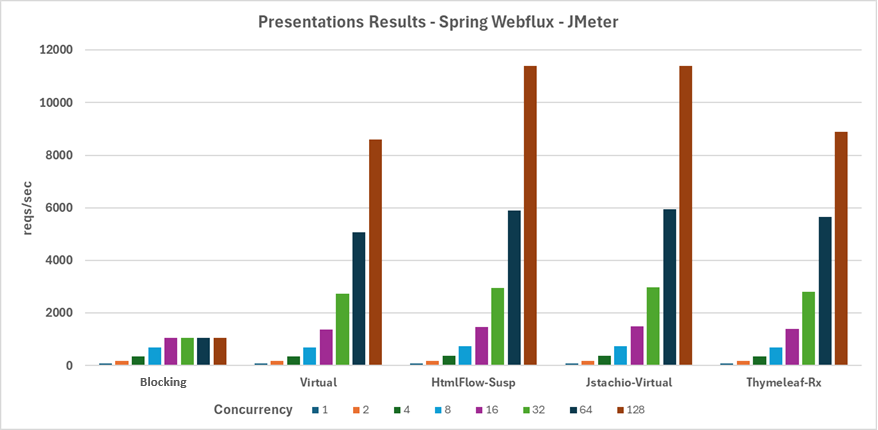
\includegraphics[width=0.8\textwidth]{./Graphs/presentations-webflux-jmeter.png}
     \caption{Presentation Benchmark Results in Spring WebFlux with JMeter}\label{fig:presentations-webflux-jmeter}
\end{figure}

The results show that when using the blocking template engines with a separate
coroutine dispatcher, the engines are unable to scale effectively beyond 16
concurrent users. In contrast, the non-blocking engines scale effectively up to
128 concurrent users, with HtmlFlow achieving approximately 11,000 requests per
second. When using the blocking approaches in the context of Virtual Threads
(achieving non-blocking I/O), the engines scale effectively up to 128
concurrent users, with Jstachio matching HtmlFlow`s performance at
approximately 11,000 requests per second. Thymeleaf, using the reactive View
Resolver driver, also scales to 128 users, albeit less effectively, achieving
around 8,500 requests per second.

\begin{figure}[h]
     \centering
     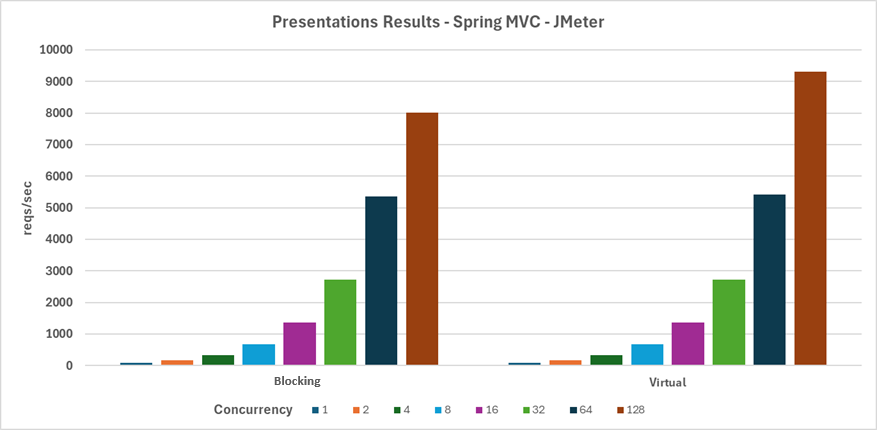
\includegraphics[width=0.8\textwidth]{./Graphs/presentations-springmvc-jmeter.png}
     \caption{Presentation Benchmark Results in Spring MVC with JMeter}\label{fig:presentations-springmvc-jmeter}
\end{figure}

The results for the Spring MVC implementation, shown in
Figure~\ref{fig:presentations-springmvc-jmeter}, compare two approaches:
\textit{Sync}, which uses platform threads with \texttt{StreamingResponseBody},
and \textit{Virtual}, which uses Virtual Threads. Both approaches scale
effectively up to 128 concurrent users, with the Virtual Thread approach
achieving a slightly higher throughput of 9,000 requests per second. However,
these values are slightly lower than those observed in the Spring WebFlux
implementation.

\begin{figure}[h]
     \centering
     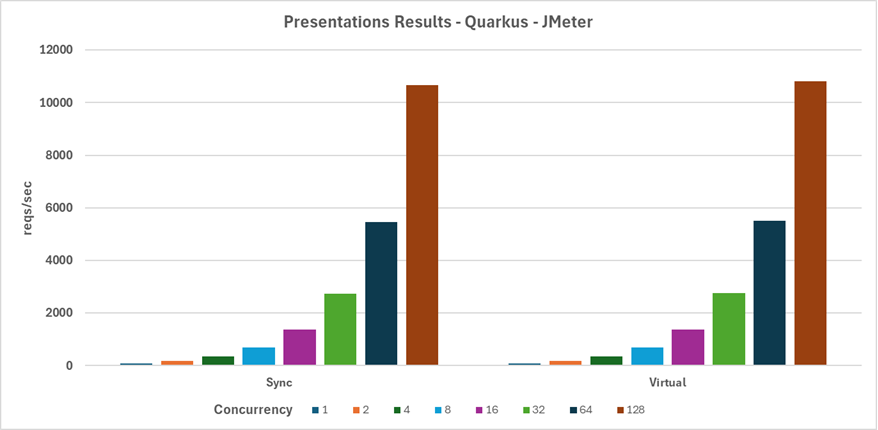
\includegraphics[width=0.8\textwidth]{./Graphs/presentations-quarkus-jmeter.png}
     \caption{Presentation Benchmark Results in Quarkus with JMeter}\label{fig:presentations-quarkus-jmeter}
\end{figure}

The results for the Quarkus implementation, shown in
Figure~\ref{fig:presentations-quarkus-jmeter} demonstrate that Quarkus handles
blocking approaches more effectively than Spring WebFlux, with the blocking
engines scaling up to 128 concurrent users and achieving 10,000 requests per
second. While the use of Virtual Threads results in a slightly higher
throughput, the difference is not significant, as both approaches deliver
similar performance.

\subsection{Stocks Results}

\begin{figure}[h]
     \centering
     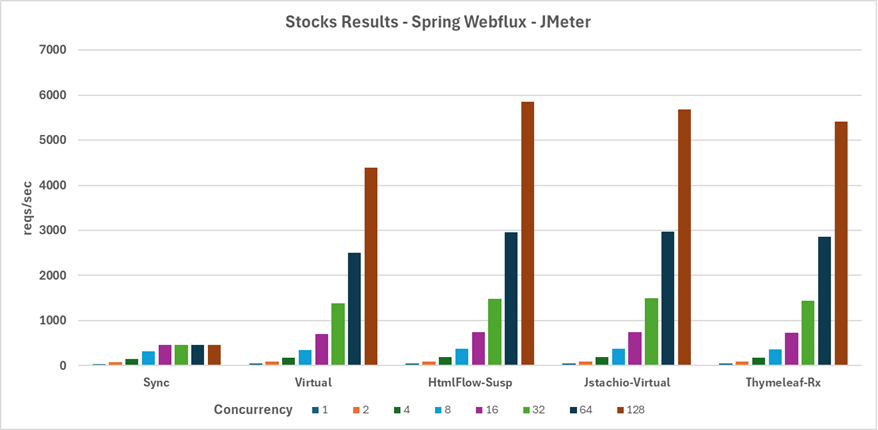
\includegraphics[width=0.8\textwidth]{./Graphs/stocks-webflux-jmeter.png}
     \caption{Stocks Benchmark Results in Spring WebFlux with JMeter}\label{fig:stocks-webflux-jmeter}
\end{figure}

The results in Figure~\ref{fig:stocks-webflux-jmeter} use the same template
engines and approaches as the previous benchmark, but replace the data model
with the more complex Stock class, including 20 instances. Despite the
increased complexity and number of instances, the scalability of the engines
remains largely unaffected. However, throughput is reduced by approximately 50
percent across all engines, with HtmlFlow achieving 6,000 requests per second.
The Thymeleaf implementation using the reactive View Resolver driver reaches
5,000 requests per second, suggesting that the performance drop compared to the
Presentation benchmark is not substantial.


\begin{figure}[h]
     \centering
     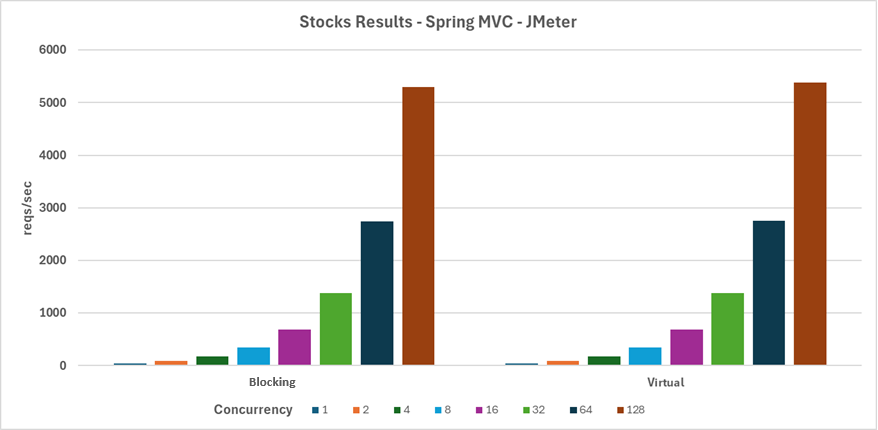
\includegraphics[width=0.8\textwidth]{./Graphs/stocks-springmvc-jmeter.png}
     \caption{Stocks Benchmark Results in Spring MVC with JMeter}\label{fig:stocks-springmvc-jmeter}
\end{figure}

The results observed in Figure~\ref{fig:stocks-springmvc-jmeter} show that the
Spring MVC implementation using the blocking approach with
\texttt{StreamingResponseBody} achieves a throughput of up to 5500 requests per
second, while no significant change is observed when using Virtual Threads. As
such, both approaches scale effectively up to 128 concurrent users.

\begin{figure}[h]
     \centering
     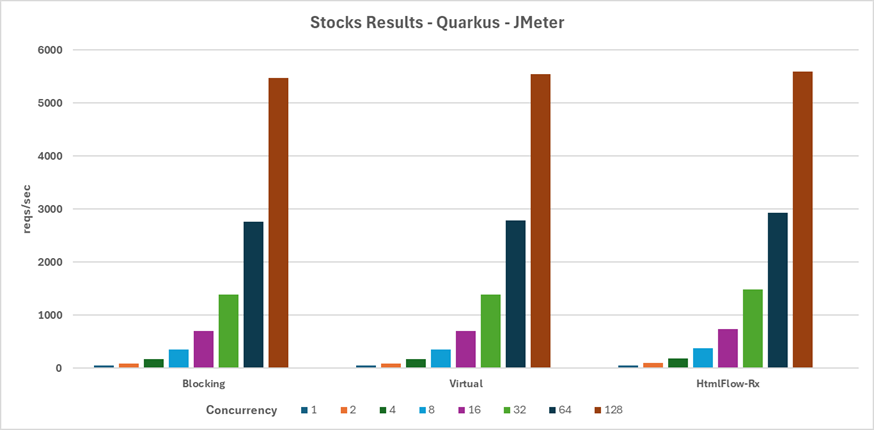
\includegraphics[width=0.8\textwidth]{./Graphs/stocks-quarkus-jmeter.png}
     \caption{Stocks Benchmark Results in Quarkus with JMeter}\label{fig:stocks-quarkus-jmeter}
\end{figure}

The results depicted in Figure~\ref{fig:stocks-quarkus-jmeter} show that the
Quarkus implementation scales effectively up to 128 concurrent users, achieving
performance comparable to the Spring WebFlux implementation. The blocking
engines reach 6,000 requests per second. Again, there is no significant
difference between the Virtual Threads and platform threads approaches, with
both achieving similar results.

The results of the benchmarks show that non-blocking engines, through the use
of reactive programming, Kotlin coroutines, or Java virtual threads, are able
to scale effectively up to 128 concurrent users. Out of all the tested
frameworks, Spring Webflux showed itself the most effective at enabling PSSR,
mostly due to its native support for Publish and Subscriber interfaces, which
allow for HTML content to be progressively streamed to the client. Quarkus also
enabled PSSR effectively, but it required additional configuration of the
\texttt{OutputBuffer} size to achieve the same results as Spring Webflux. The
Spring MVC implementation, on the other hand, did not enable PSSR for the
tested templates.

Additionally, the results show that approaches using Virtual Threads are able
to scale as effectively as those using reactive programming or Kotlin
coroutines, with the advantage of being easier to implement and understand for 
developers. 

\section{Conclusion}

In recent decades, non-blocking I/O has become the standard approach for building
highly responsive and scalable web servers. However, traditional synchronous
programming models are not compatible with non-blocking APIs, which typically
rely on callback-based conventions such as
\textit{continuation-passing style} (CPS)~\cite{scheme} or
\textit{promises}~\cite{promise}. These approaches not only hinder
sequential readability but also increase code verbosity, making them more
error-prone.
Alternatives like the \texttt{async}/\texttt{await} idiom~\cite{async_await}
or \textit{suspend functions}~\cite{elizarov2021coroutines} simplify
asynchronous programming by mimicking a sequential style without blocking
threads.
Recent proposals~\cite{carvalho2023async,wise2024pssr} have applied contemporary
asynchronous idioms to SSR web templates, demonstrating how they can overcome
the scalability bottlenecks present in traditional web template engines.

As an alternative, Java Virtual Threads can be applied to any blocking I/O call,
leveraging the Java runtime to transparently intercept and convert it into non-blocking I/O,
without requiring any changes to the calling code or exposing its internal complexities.
In this work, we explored how this technique can be applied to traditional
web template engines and whether it can achieve performance competitive with
reactive approaches provided by frameworks such as Thymeleaf~\cite{webflux} and HtmlFlow~\cite{htmlflow}.
Our benchmarks across Spring WebFlux, Spring MVC, and Quarkus show that synchronous
non-blocking execution using virtual threads consistently delivers performance
comparable to asynchronous non-blocking approaches under high concurrency.
These findings highlight virtual threads as a promising alternative to complex
asynchronous programming models, offering a simpler development experience
without compromising scalability or responsiveness.

% 
% All figures and tables should be cited in the main text as Figure~\ref{fig1},
% Table~\ref{tab1}, etc.
% 
% \begin{figure}[H]
% 	%\isPreprints{\centering}{} % Only used for preprints
% 	
\includegraphics[width=4 cm]{Definitions/logo-mdpi}
% 	\caption{This is a figure. Schemes follow the same formatting.\label{fig1}}
% \end{figure}
% \unskip
% 
% % Example of a figure that spans the whole page width and with subfigures. The same concept works for tables, too.
% \begin{figure}[H]
% 	%\isPreprints{}{% This command is only used for ``preprints''.
% 	\begin{adjustwidth}{-\extralength}{0cm}
% 		\centering
% 		%} % If the paper is ``preprints'', please uncomment this parenthesis.
% 		\subfloat[\centering]{
\includegraphics[width=7.0cm]{Definitions/logo-mdpi}}
% 		%\hfill
% 		\subfloat[\centering]{
\includegraphics[width=7.0cm]{Definitions/logo-mdpi}}\\
% 		\subfloat[\centering]{
\includegraphics[width=7.0cm]{Definitions/logo-mdpi}}
% 		%\hfill
% 		\subfloat[\centering]{
\includegraphics[width=7.0cm]{Definitions/logo-mdpi}}
% 		%\isPreprints{}{% This command is only used for ``preprints''.
% 	\end{adjustwidth}
% 	%} % If the paper is ``preprints'', please uncomment this parenthesis.
% 	\caption{This is a wide figure. Schemes follow the same formatting. If there are multiple panels, they should be listed as: (\textbf{a}) Description of what is contained in the first panel. (\textbf{b}) Description of what is contained in the second panel. (\textbf{c}) Description of what is contained in the third panel. (\textbf{d}) Description of what is contained in the fourth panel. Figures should be placed in the main text near to the first time they are cited. A caption on a single line should be centered.\label{fig2}}
% \end{figure}
% 
% \begin{table}[H]
% 	\caption{This is a wide table.\label{tab2}}
% 	%\isPreprints{\centering}{% This command is only used for ``preprints''.
% 	\begin{adjustwidth}{-\extralength}{0cm}
% 		%} % If the paper is ``preprints'', please uncomment this parenthesis.
% 		%\isPreprints{\begin{tabularx}{\textwidth}{CCCC}}{% This command is only used for ``preprints''.
% 		\begin{tabularx}{\fulllength}{CCCC}
% 			%} % If the paper is ``preprints'', please uncomment this parenthesis.
% 			\toprule
% 			\textbf{Title 1}              & \textbf{Title 2} & \textbf{Title 3} & \textbf{Title 4} \\
% 			\midrule
% 			\multirow[m]{3}{*}{Entry 1 *} & Data             & Data             & Data             \\
% 			                              & Data             & Data             & Data             \\
% 			                              & Data             & Data             & Data             \\
% 			\midrule
% 			\multirow[m]{3}{*}{Entry 2}   & Data             & Data             & Data             \\
% 			                              & Data             & Data             & Data             \\
% 			                              & Data             & Data             & Data             \\
% 			\bottomrule
% 		\end{tabularx}
% 		%		\isPreprints{}{% This command is only used for ``preprints''.
% 	\end{adjustwidth}
% 	%} % If the paper is ``preprints'', please uncomment this parenthesis.
% 	\noindent{\footnotesize{* Tables may have a footer.}}
% \end{table}
% 
%\begin{listing}[H]
%\caption{Title of the listing}
%\rule{\columnwidth}{1pt}
%\raggedright Text of the listing. In font size footnotesize, small, or normalsize. Preferred format: left aligned and single spaced. Preferred border format: top border line and bottom border line.
%\rule{\columnwidth}{1pt}
%\end{listing}

%%%%%%%%%%%%%%%%%%%%%%%%%%%%%%%%%%%%%%%%%%
% \section{Conclusions}
% 
% This section is not mandatory, but can be added to the manuscript if the
% discussion is unusually long or complex.

%%%%%%%%%%%%%%%%%%%%%%%%%%%%%%%%%%%%%%%%%%
\vspace{6pt}

%%%%%%%%%%%%%%%%%%%%%%%%%%%%%%%%%%%%%%%%%%
%% optional
%\supplementary{The following supporting information can be downloaded at:  \linksupplementary{s1}, Figure S1: title; Table S1: title; Video S1: title.}

% Only for journal Methods and Protocols:
% If you wish to submit a video article, please do so with any other supplementary material.
% \supplementary{The following supporting information can be downloaded at: \linksupplementary{s1}, Figure S1: title; Table S1: title; Video S1: title. A supporting video article is available at doi: link.}

% Only used for preprtints:
% \supplementary{The following supporting information can be downloaded at the website of this paper posted on \href{https://www.preprints.org/}{Preprints.org}.}

% Only for journal Hardware:
% If you wish to submit a video article, please do so with any other supplementary material.
% \supplementary{The following supporting information can be downloaded at: \linksupplementary{s1}, Figure S1: title; Table S1: title; Video S1: title.\vspace{6pt}\\
%\begin{tabularx}{\textwidth}{lll}
%\toprule
%\textbf{Name} & \textbf{Type} & \textbf{Description} \\
%\midrule
%S1 & Python script (.py) & Script of python source code used in XX \\
%S2 & Text (.txt) & Script of modelling code used to make Figure X \\
%S3 & Text (.txt) & Raw data from experiment X \\
%S4 & Video (.mp4) & Video demonstrating the hardware in use \\
%... & ... & ... \\
%\bottomrule
%\end{tabularx}
%}

%%%%%%%%%%%%%%%%%%%%%%%%%%%%%%%%%%%%%%%%%%
\authorcontributions{`Conceptualization, X.X. and Y.Y.; methodology, X.X.; software, X.X.; validation, X.X., Y.Y. and Z.Z.; formal analysis, X.X.; investigation, X.X.; resources, X.X.; data curation, X.X.; writing---original draft preparation, X.X.; writing---review and editing, X.X.; visualization, X.X.; supervision, X.X.; project administration, X.X.; funding acquisition, Y.Y. All authors have read and agreed to the published version of the manuscript., please turn to the  \href{http://img.mdpi.org/data/contributor-role-instruction.pdf}{CRediT taxonomy} for the term explanation. Authorship must be limited to those who have contributed substantially to the work~reported.}

\funding{This research received no external funding}

\institutionalreview{Not applicable.}

\dataavailability{We encourage all authors of articles published in MDPI journals to share their research data. In this section, please provide details regarding where data supporting reported results can be found, including links to publicly archived datasets analyzed or generated during the study. Where no new data were created, or where data is unavailable due to privacy or ethical restrictions, a statement is still required. Suggested Data Availability Statements are available in section ``MDPI Research Data Policies'' at \url{https://www.mdpi.com/ethics}.}

% Only for journal Drones
%\durcstatement{Current research is limited to the [please insert a specific academic field, e.g., XXX], which is beneficial [share benefits and/or primary use] and does not pose a threat to public health or national security. Authors acknowledge the dual-use potential of the research involving xxx and confirm that all necessary precautions have been taken to prevent potential misuse. As an ethical responsibility, authors strictly adhere to relevant national and international laws about DURC. Authors advocate for responsible deployment, ethical considerations, regulatory compliance, and transparent reporting to mitigate misuse risks and foster beneficial outcomes.}

% Only for journal Nursing Reports
%\publicinvolvement{Please describe how the public (patients, consumers, carers) were involved in the research. Consider reporting against the GRIPP2 (Guidance for Reporting Involvement of Patients and the Public) checklist. If the public were not involved in any aspect of the research add: ``No public involvement in any aspect of this research''.}
%
%% Only for journal Nursing Reports
%\guidelinesstandards{Please add a statement indicating which reporting guideline was used when drafting the report. For example, ``This manuscript was drafted against the XXX (the full name of reporting guidelines and citation) for XXX (type of research) research''. A complete list of reporting guidelines can be accessed via the equator network: \url{https://www.equator-network.org/}.}
%
%% Only for journal Nursing Reports
%\useofartificialintelligence{Please describe in detail any and all uses of artificial intelligence (AI) or AI-assisted tools used in the preparation of the manuscript. This may include, but is not limited to, language translation, language editing and grammar, or generating text. Alternatively, please state that “AI or AI-assisted tools were not used in drafting any aspect of this manuscript”.}

\conflictsofinterest{Declare conflicts of interest or state ``The authors declare no conflicts of interest.'' Authors must identify and declare any personal circumstances or interest that may be perceived as inappropriately influencing the representation or interpretation of reported research results. Any role of the funders in the design of the study; in the collection, analyses or interpretation of data; in the writing of the manuscript; or in the decision to publish the results must be declared in this section. If there is no role, please state ``The funders had no role in the design of the study; in the collection, analyses, or interpretation of data; in the writing of the manuscript; or in the decision to publish the results''.}

%%%%%%%%%%%%%%%%%%%%%%%%%%%%%%%%%%%%%%%%%%
%\isPreprints{} % If the paper is ``preprints'', please uncomment this parenthesis.
	%\printendnotes[custom] % Un-comment to print a list of endnotes

	\reftitle{References}

	% Please provide either the correct journal abbreviation (e.g. according to the “List of Title Word Abbreviations” http://www.issn.org/services/online-services/access-to-the-ltwa/) or the full name of the journal.
	% Citations and References in Supplementary files are permitted provided that they also appear in the reference list here. 

	%=====================================
	% References, variant A: external bibliography
	%=====================================
	\bibliography{referencias.bib}

	%=====================================
	% References, variant B: internal bibliography
	%=====================================

	\PublishersNote{}
	%\isPreprints{} % If the paper is ``preprints'', please uncomment this parenthesis.
\end{document}

